\chapter*{Introduction}


In the aurora 2020-2021 for USA and maybe before, like 2019 for Chinese supercomputers, the world will reach another milestone in the power of machines, the Exascale. 
This supercomputer will be $100$ times faster than the estimated overfall operations performed by the human brain and its $10^{16}$ \textbf{FL}oating point \textbf{O}perations \textbf{P}er \textbf{S}econd (FLOPS) and reach a computational power of a trillion ($10^{18}$) FLOPS.

This odyssey started long time ago with the first vacuum tubes and the need of balistic in war. 
Nowdays the main aim does not changed a lot and the power of a nation is represented by its army but also the computational power of its supercomputers. 
Since 1962, considering the Cray CDC 6600 as the first supercomputer, the power of those machines have increase following an observation of the co-fonder of the Intel company, Alan Moore. 
Better known under as the "Moore's Law" it speculates in 1965 that considering the evoluation of technology the number of transistors on a dense integrated circuit will double approximately every two years. 
Thus the computational power, that depend intrinsectly of the number of processors on the chip, will also increase. 
This observation can be related to the supercomputers results through the years in the TOP500 list. 
\begin{figure}
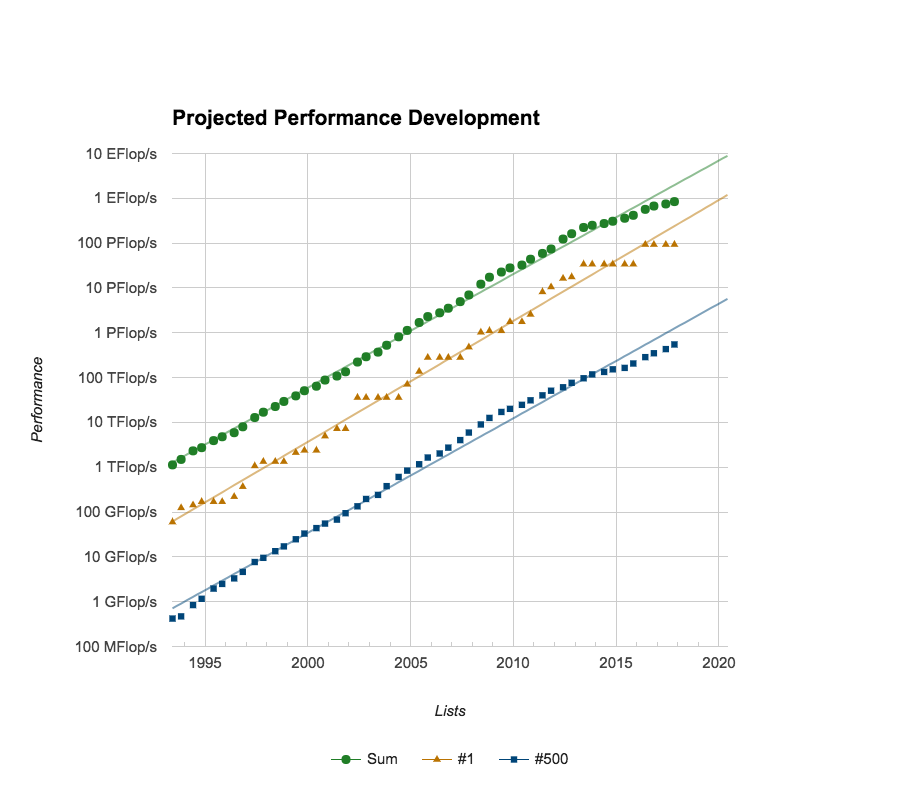
\includegraphics[width=\linewidth]{figures/introduction/top500_list_approximation.png}
\caption{Computational power evolution in the TOP500 list}
\label{fig:intro_top500}
\end{figure}

As shown on figure \ref{fig:intro_top500}, even if estimated in early 1965, the Moore's law seems to be accurate. 

Those good results are not just gave by the shrink in the semiconductor with smaller transistors.
At some point in early tweenty century IBM proposed the first multi-core processor.
The constructors started then to propose chips with more than one core to increase the computational power in conjonction with the shrink of semiconductors, allowing the Moore's law to thirve. 
This increase of the overall power of the chip comes with some complementary cost in synchronizations steps between the chips for memory access, work sharing and of course the power consumption.
The general purpose CPU usually features from 2 to 16 cores on a single ship. 

But since 2013-2014 a lot of companies, like Intel the Gordon Moore's company, stated that this law is over. 
This can be see on figure \ref{fig:intro_top500}, in the right part of the graph, the evolution is not linear anymore and tend to dicrease. 
This is due to two main factors: on one hand, we slowly reach the maximal shrink size of the transistors implying hard to handle side effects and on another hand the power wall implyed by the power consumption required by so many transistors and frequency speed on the chip.
And some ways were found years before to overcome this again using many-cores architectures which are now called accelerstors. 
Companies like Intel, NVIDIA, AMD, Altera propose their accelerator going from Xeon Phi, General Purpose Graphics Processing Unit (GPGPU) initialy used in graphics, Field Programmable Gates Array (FPGA) or even dedicated Application-Specific Integrated Circuit (ASIC).
Those architecture takes the chose to implement very simple cores with low power consumption used by thousand in the same chip. 
This add an extrat cost in the synchronization and coordination on chip and add a need for specified memory. 
Those Devices, for most of them, also need to be controlled by a Host CPU adding another extra cost to shared data between the Host and Device. 
But used efficiently with fitting massively parallel applications, they can release a computational power way better than the classical CPU. 

Even with these devices, nowaday supercomputers are facing several problems in their conception and utilization. 
The three mains are the power wall, the communication wall and the memory wall bounding the overall computional power of the machines.  
Some subproblems like the the interconnect wall, resilience wall or even the complexity wall also arise and make the task even harder.\\

This is were this study take place, how to use those accelerators or devices in the right way and are they the way that will help us the reach exascale.
We considered that the classical TOP500 ranking is not enough to target all the main wall problems of those architectures and especially accelerators. 
Indeed it is based on LINPACK/LAPACK with regular computation and communication that perfectly fit this architecture and does not show the reality that the domain scientists have to face in their simulation. 

We propose a metric that extracts the three main issues of HPC and applyed them on accelerators architectures to figure out how to take advantage of those architectures and what are the limitations. 
This study is decomposed in 3 problems. The first two are targeting computation and communication wall over very irregular cases with high memory accesses, using an academic combinatorial problem and the Graph500 benchmark. 
The last is a computational scientific problem that cover both of the problems and appears to be hard to implement on supercomputers and even more on accelerated ones.\\

This thesis is composed of 3 chapters. 
The first will develope the state of the art in HPC from the main law to the hardware. 
We describe how the nowaday supercomputers are ranked and what are the main walls in their evoluiton. \\

In the second chapter we propose our metric to characterize supercomputers architectures. 
The Langford problem is described as an irregular and computationally heavy problem.
This shows how the accelerators, in this case GPU, are able to support the memory and computation wall. 
This allowed us to beat a world record on the last instances of this academic problem.
The Graph500 problem is then proposed as an irregular and communications heavy problem. 
We present our implementation and the logic to take advantage of the GPU computational power in an \\

Then, in the last chapter, we consider a problem that is heavy and irregular regarding to computation and communications.
This problem is the milestone of our metric and show how nowadays supercomputers can overcome those issues. 
This computational science problem is based on the SPH method and we intend to provide a tool for Physisists and Astrophysists and is called FleCSPH. \\

The last part will conclude on this work and results and show some of the main prospects of this study and my future researches. 